\section{Restrições, Assumptions e Custos}

\subsection{Restrições}

\begin{itemize}
  \item Prazo Académico
  \begin{itemize}
    \item Prazo de entrega final limitado e imutável, definida pelo calendário académico.
    \item Tempo limitado para o desenvolvimento, experimentação, análise de resultados e redação de documentos necessários.
  \end{itemize}

  \item Conformidade Ética e de Segurança
  \begin{itemize}
    \item Cumprimento integral de normas éticas na experimentação com LLMs, assegurando que a geração de conteúdo malicioso é apenas para fins de benchmarking em ambiente controlado.
    \item Garantia de que todos os dados utilizados respeitam as políticas de privacidade e os direitos de autor.
  \end{itemize}

  \item Recursos Computacionais
  \begin{itemize}
    \item Limitações de hardware local (ex: memória GPU, capacidade de processamento) para executar modelos grandes.
    \item Dependência de ferramentas e plataformas externas (ex: Ollama, PyRIT) que podem impor limites de desempenho ou disponibilidade.
  \end{itemize}

  \item Âmbito do Projeto
  \begin{itemize}
    \item Foco exclusivo no benchmarking de segurança de LLMs no contexto de geração de código vulnerável e malicioso.
    \item Exclusão explícita de outros tipos de ataques (ex: deepfakes, desinformação) ou contextos não relacionados com código.
  \end{itemize}

  \item Acesso a Modelos
  \begin{itemize}
    \item Dependência da disponibilidade e acesso a modelos específicos de LLMs, cujas versões ou licenças podem mudar.
    \item Possíveis restrições de licenciamento em modelos proprietários que limitem a escala dos testes.
  \end{itemize}
\end{itemize}

\subsection{Assumptions}

\begin{itemize}
  \item Recursos Computacionais: Existência de uma VM com recursos suficientes para executar LLMs locais.
  \item Acesso a Modelos: Os modelos de LLM selecionados permanecerão disponíveis e acessíveis.
\end{itemize}

\subsection{Custos}

Nesta secção é apresentada a previsão dos custos associados ao projeto, incluindo a estimativa global e por tarefa. A Figura~\ref{fig:costs_overal_estimation} mostra a estimativa geral do custo e a Figura~\ref{fig:individual_task_estimatioion} apresenta a estimativa individual de cada tarefa.

\begin{figure}[H]
    \centering
    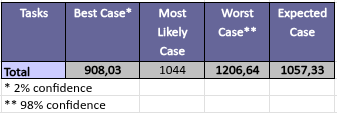
\includegraphics[width=0.5\textwidth]{images/costs_overal_estimation.png}
    \caption{Estimatimativa Geral do Custo}
    \label{fig:costs_overal_estimation}
\end{figure}

\begin{figure}[H]
    \centering
    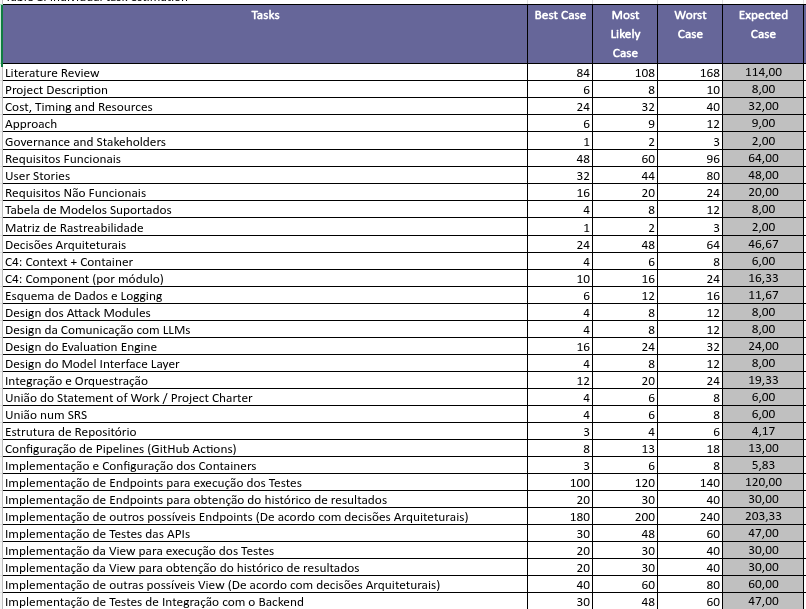
\includegraphics[width=0.8\textwidth]{images/individual_task_estimatioion.png}
    \caption{Estimatimativa Individual de Cada Tarefa}
    \label{fig:individual_task_estimatioion}
\end{figure}
